%\documentclass{standalone}
%\usepackage{tikz}
%\usetikzlibrary{patterns,plotmarks}
%\begin{document}
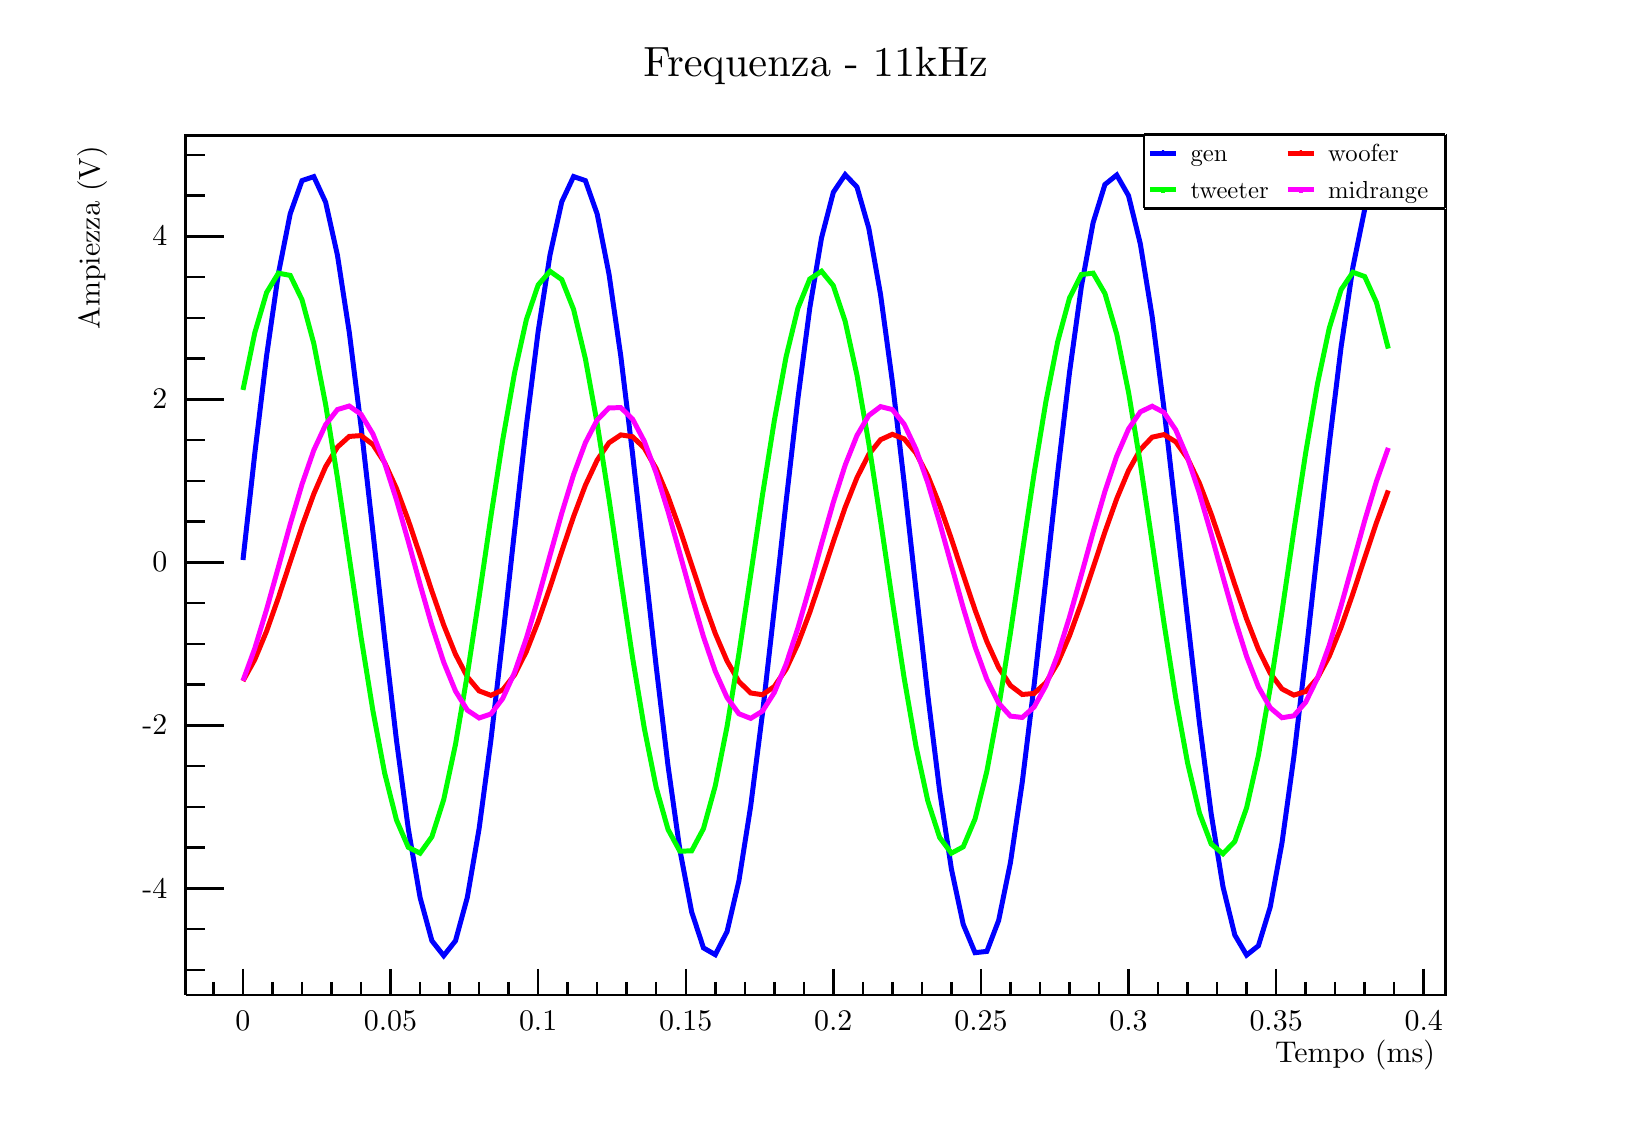
\begin{tikzpicture}
\def\CheckTikzLibraryLoaded#1{ \ifcsname tikz@library@#1@loaded\endcsname \else \PackageWarning{tikz}{usetikzlibrary{#1} is missing in the preamble.} \fi }
\CheckTikzLibraryLoaded{patterns}
\CheckTikzLibraryLoaded{plotmarks}
\pgfdeclareplotmark{cross} {
\pgfpathmoveto{\pgfpoint{-0.3\pgfplotmarksize}{\pgfplotmarksize}}
\pgfpathlineto{\pgfpoint{+0.3\pgfplotmarksize}{\pgfplotmarksize}}
\pgfpathlineto{\pgfpoint{+0.3\pgfplotmarksize}{0.3\pgfplotmarksize}}
\pgfpathlineto{\pgfpoint{+1\pgfplotmarksize}{0.3\pgfplotmarksize}}
\pgfpathlineto{\pgfpoint{+1\pgfplotmarksize}{-0.3\pgfplotmarksize}}
\pgfpathlineto{\pgfpoint{+0.3\pgfplotmarksize}{-0.3\pgfplotmarksize}}
\pgfpathlineto{\pgfpoint{+0.3\pgfplotmarksize}{-1.\pgfplotmarksize}}
\pgfpathlineto{\pgfpoint{-0.3\pgfplotmarksize}{-1.\pgfplotmarksize}}
\pgfpathlineto{\pgfpoint{-0.3\pgfplotmarksize}{-0.3\pgfplotmarksize}}
\pgfpathlineto{\pgfpoint{-1.\pgfplotmarksize}{-0.3\pgfplotmarksize}}
\pgfpathlineto{\pgfpoint{-1.\pgfplotmarksize}{0.3\pgfplotmarksize}}
\pgfpathlineto{\pgfpoint{-0.3\pgfplotmarksize}{0.3\pgfplotmarksize}}
\pgfpathclose
\pgfusepathqstroke
}
\pgfdeclareplotmark{cross*} {
\pgfpathmoveto{\pgfpoint{-0.3\pgfplotmarksize}{\pgfplotmarksize}}
\pgfpathlineto{\pgfpoint{+0.3\pgfplotmarksize}{\pgfplotmarksize}}
\pgfpathlineto{\pgfpoint{+0.3\pgfplotmarksize}{0.3\pgfplotmarksize}}
\pgfpathlineto{\pgfpoint{+1\pgfplotmarksize}{0.3\pgfplotmarksize}}
\pgfpathlineto{\pgfpoint{+1\pgfplotmarksize}{-0.3\pgfplotmarksize}}
\pgfpathlineto{\pgfpoint{+0.3\pgfplotmarksize}{-0.3\pgfplotmarksize}}
\pgfpathlineto{\pgfpoint{+0.3\pgfplotmarksize}{-1.\pgfplotmarksize}}
\pgfpathlineto{\pgfpoint{-0.3\pgfplotmarksize}{-1.\pgfplotmarksize}}
\pgfpathlineto{\pgfpoint{-0.3\pgfplotmarksize}{-0.3\pgfplotmarksize}}
\pgfpathlineto{\pgfpoint{-1.\pgfplotmarksize}{-0.3\pgfplotmarksize}}
\pgfpathlineto{\pgfpoint{-1.\pgfplotmarksize}{0.3\pgfplotmarksize}}
\pgfpathlineto{\pgfpoint{-0.3\pgfplotmarksize}{0.3\pgfplotmarksize}}
\pgfpathclose
\pgfusepathqfillstroke
}
\pgfdeclareplotmark{newstar} {
\pgfpathmoveto{\pgfqpoint{0pt}{\pgfplotmarksize}}
\pgfpathlineto{\pgfqpointpolar{44}{0.5\pgfplotmarksize}}
\pgfpathlineto{\pgfqpointpolar{18}{\pgfplotmarksize}}
\pgfpathlineto{\pgfqpointpolar{-20}{0.5\pgfplotmarksize}}
\pgfpathlineto{\pgfqpointpolar{-54}{\pgfplotmarksize}}
\pgfpathlineto{\pgfqpointpolar{-90}{0.5\pgfplotmarksize}}
\pgfpathlineto{\pgfqpointpolar{234}{\pgfplotmarksize}}
\pgfpathlineto{\pgfqpointpolar{198}{0.5\pgfplotmarksize}}
\pgfpathlineto{\pgfqpointpolar{162}{\pgfplotmarksize}}
\pgfpathlineto{\pgfqpointpolar{134}{0.5\pgfplotmarksize}}
\pgfpathclose
\pgfusepathqstroke
}
\pgfdeclareplotmark{newstar*} {
\pgfpathmoveto{\pgfqpoint{0pt}{\pgfplotmarksize}}
\pgfpathlineto{\pgfqpointpolar{44}{0.5\pgfplotmarksize}}
\pgfpathlineto{\pgfqpointpolar{18}{\pgfplotmarksize}}
\pgfpathlineto{\pgfqpointpolar{-20}{0.5\pgfplotmarksize}}
\pgfpathlineto{\pgfqpointpolar{-54}{\pgfplotmarksize}}
\pgfpathlineto{\pgfqpointpolar{-90}{0.5\pgfplotmarksize}}
\pgfpathlineto{\pgfqpointpolar{234}{\pgfplotmarksize}}
\pgfpathlineto{\pgfqpointpolar{198}{0.5\pgfplotmarksize}}
\pgfpathlineto{\pgfqpointpolar{162}{\pgfplotmarksize}}
\pgfpathlineto{\pgfqpointpolar{134}{0.5\pgfplotmarksize}}
\pgfpathclose
\pgfusepathqfillstroke
}
\definecolor{c}{rgb}{1,1,1};
\draw [color=c, fill=c] (0,0) rectangle (20,13.639);
\draw [color=c, fill=c] (2,1.3639) rectangle (18,12.2751);
\definecolor{c}{rgb}{0,0,0};
\draw [c,line width=0.9] (2,1.3639) -- (2,12.2751) -- (18,12.2751) -- (18,1.3639) -- (2,1.3639);
\definecolor{c}{rgb}{1,1,1};
\draw [color=c, fill=c] (2,1.3639) rectangle (18,12.2751);
\definecolor{c}{rgb}{0,0,0};
\draw [c,line width=0.9] (2,1.3639) -- (2,12.2751) -- (18,12.2751) -- (18,1.3639) -- (2,1.3639);
\draw [c,line width=0.9] (2,1.3639) -- (18,1.3639);
\draw [c,line width=0.9] (2.72727,1.69123) -- (2.72727,1.3639);
\draw [c,line width=0.9] (3.10216,1.52756) -- (3.10216,1.3639);
\draw [c,line width=0.9] (3.47704,1.52756) -- (3.47704,1.3639);
\draw [c,line width=0.9] (3.85192,1.52756) -- (3.85192,1.3639);
\draw [c,line width=0.9] (4.2268,1.52756) -- (4.2268,1.3639);
\draw [c,line width=0.9] (4.60169,1.69123) -- (4.60169,1.3639);
\draw [c,line width=0.9] (4.97657,1.52756) -- (4.97657,1.3639);
\draw [c,line width=0.9] (5.35145,1.52756) -- (5.35145,1.3639);
\draw [c,line width=0.9] (5.72634,1.52756) -- (5.72634,1.3639);
\draw [c,line width=0.9] (6.10122,1.52756) -- (6.10122,1.3639);
\draw [c,line width=0.9] (6.4761,1.69123) -- (6.4761,1.3639);
\draw [c,line width=0.9] (6.85098,1.52756) -- (6.85098,1.3639);
\draw [c,line width=0.9] (7.22587,1.52756) -- (7.22587,1.3639);
\draw [c,line width=0.9] (7.60075,1.52756) -- (7.60075,1.3639);
\draw [c,line width=0.9] (7.97563,1.52756) -- (7.97563,1.3639);
\draw [c,line width=0.9] (8.35052,1.69123) -- (8.35052,1.3639);
\draw [c,line width=0.9] (8.7254,1.52756) -- (8.7254,1.3639);
\draw [c,line width=0.9] (9.10028,1.52756) -- (9.10028,1.3639);
\draw [c,line width=0.9] (9.47516,1.52756) -- (9.47516,1.3639);
\draw [c,line width=0.9] (9.85005,1.52756) -- (9.85005,1.3639);
\draw [c,line width=0.9] (10.2249,1.69123) -- (10.2249,1.3639);
\draw [c,line width=0.9] (10.5998,1.52756) -- (10.5998,1.3639);
\draw [c,line width=0.9] (10.9747,1.52756) -- (10.9747,1.3639);
\draw [c,line width=0.9] (11.3496,1.52756) -- (11.3496,1.3639);
\draw [c,line width=0.9] (11.7245,1.52756) -- (11.7245,1.3639);
\draw [c,line width=0.9] (12.0993,1.69123) -- (12.0993,1.3639);
\draw [c,line width=0.9] (12.4742,1.52756) -- (12.4742,1.3639);
\draw [c,line width=0.9] (12.8491,1.52756) -- (12.8491,1.3639);
\draw [c,line width=0.9] (13.224,1.52756) -- (13.224,1.3639);
\draw [c,line width=0.9] (13.5989,1.52756) -- (13.5989,1.3639);
\draw [c,line width=0.9] (13.9738,1.69123) -- (13.9738,1.3639);
\draw [c,line width=0.9] (14.3486,1.52756) -- (14.3486,1.3639);
\draw [c,line width=0.9] (14.7235,1.52756) -- (14.7235,1.3639);
\draw [c,line width=0.9] (15.0984,1.52756) -- (15.0984,1.3639);
\draw [c,line width=0.9] (15.4733,1.52756) -- (15.4733,1.3639);
\draw [c,line width=0.9] (15.8482,1.69123) -- (15.8482,1.3639);
\draw [c,line width=0.9] (16.2231,1.52756) -- (16.2231,1.3639);
\draw [c,line width=0.9] (16.5979,1.52756) -- (16.5979,1.3639);
\draw [c,line width=0.9] (16.9728,1.52756) -- (16.9728,1.3639);
\draw [c,line width=0.9] (17.3477,1.52756) -- (17.3477,1.3639);
\draw [c,line width=0.9] (17.7226,1.69123) -- (17.7226,1.3639);
\draw [c,line width=0.9] (2.72727,1.69123) -- (2.72727,1.3639);
\draw [c,line width=0.9] (2.35239,1.52756) -- (2.35239,1.3639);
\draw [c,line width=0.9] (17.7226,1.69123) -- (17.7226,1.3639);
\draw [anchor=base] (2.72727,0.913811) node[scale=1.08185, color=c, rotate=0]{0};
\draw [anchor=base] (4.60169,0.913811) node[scale=1.08185, color=c, rotate=0]{0.05};
\draw [anchor=base] (6.4761,0.913811) node[scale=1.08185, color=c, rotate=0]{0.1};
\draw [anchor=base] (8.35052,0.913811) node[scale=1.08185, color=c, rotate=0]{0.15};
\draw [anchor=base] (10.2249,0.913811) node[scale=1.08185, color=c, rotate=0]{0.2};
\draw [anchor=base] (12.0993,0.913811) node[scale=1.08185, color=c, rotate=0]{0.25};
\draw [anchor=base] (13.9738,0.913811) node[scale=1.08185, color=c, rotate=0]{0.3};
\draw [anchor=base] (15.8482,0.913811) node[scale=1.08185, color=c, rotate=0]{0.35};
\draw [anchor=base] (17.7226,0.913811) node[scale=1.08185, color=c, rotate=0]{0.4};
\draw [anchor= east] (18,0.600115) node[scale=1.08185, color=c, rotate=0]{ Tempo (ms)};
\draw [c,line width=0.9] (2,1.3639) -- (2,12.2751);
\draw [c,line width=0.9] (2.48,2.71529) -- (2,2.71529);
\draw [c,line width=0.9] (2.24,3.23287) -- (2,3.23287);
\draw [c,line width=0.9] (2.24,3.75045) -- (2,3.75045);
\draw [c,line width=0.9] (2.24,4.26804) -- (2,4.26804);
\draw [c,line width=0.9] (2.48,4.78562) -- (2,4.78562);
\draw [c,line width=0.9] (2.24,5.30321) -- (2,5.30321);
\draw [c,line width=0.9] (2.24,5.82079) -- (2,5.82079);
\draw [c,line width=0.9] (2.24,6.33837) -- (2,6.33837);
\draw [c,line width=0.9] (2.48,6.85596) -- (2,6.85596);
\draw [c,line width=0.9] (2.24,7.37354) -- (2,7.37354);
\draw [c,line width=0.9] (2.24,7.89112) -- (2,7.89112);
\draw [c,line width=0.9] (2.24,8.40871) -- (2,8.40871);
\draw [c,line width=0.9] (2.48,8.92629) -- (2,8.92629);
\draw [c,line width=0.9] (2.24,9.44388) -- (2,9.44388);
\draw [c,line width=0.9] (2.24,9.96146) -- (2,9.96146);
\draw [c,line width=0.9] (2.24,10.479) -- (2,10.479);
\draw [c,line width=0.9] (2.48,10.9966) -- (2,10.9966);
\draw [c,line width=0.9] (2.48,2.71529) -- (2,2.71529);
\draw [c,line width=0.9] (2.24,2.1977) -- (2,2.1977);
\draw [c,line width=0.9] (2.24,1.68012) -- (2,1.68012);
\draw [c,line width=0.9] (2.48,10.9966) -- (2,10.9966);
\draw [c,line width=0.9] (2.24,11.5142) -- (2,11.5142);
\draw [c,line width=0.9] (2.24,12.0318) -- (2,12.0318);
\draw [anchor= east] (1.9,2.71529) node[scale=1.08185, color=c, rotate=0]{-4};
\draw [anchor= east] (1.9,4.78562) node[scale=1.08185, color=c, rotate=0]{-2};
\draw [anchor= east] (1.9,6.85596) node[scale=1.08185, color=c, rotate=0]{0};
\draw [anchor= east] (1.9,8.92629) node[scale=1.08185, color=c, rotate=0]{2};
\draw [anchor= east] (1.9,10.9966) node[scale=1.08185, color=c, rotate=0]{4};
\draw [anchor= east] (0.812894,12.2751) node[scale=1.08185, color=c, rotate=90]{ Ampiezza (V)};
\definecolor{c}{rgb}{0,0,1};
\draw [c,line width=1.8] (2.72727,6.8855) -- (2.87723,8.2359) -- (3.02718,9.47966) -- (3.17713,10.523) -- (3.32709,11.2823) -- (3.47704,11.7034) -- (3.62699,11.7544) -- (3.77694,11.4294) -- (3.9269,10.7566) -- (4.07685,9.78065) -- (4.2268,8.58204) --
 (4.37676,7.25147) -- (4.52671,5.88958) -- (4.67666,4.59519) -- (4.82662,3.47394) -- (4.97657,2.59849) -- (5.12652,2.05002) -- (5.27648,1.85986) -- (5.42643,2.04985) -- (5.57638,2.60066) -- (5.72634,3.47477) -- (5.87629,4.60052) -- (6.02624,5.89458)
 -- (6.1762,7.2568) -- (6.32615,8.59071) -- (6.4761,9.78915) -- (6.62605,10.7584) -- (6.77601,11.4348) -- (6.92596,11.7551) -- (7.07591,11.7036) -- (7.22587,11.2789) -- (7.37582,10.5156) -- (7.52577,9.47266) -- (7.67573,8.2274) -- (7.82568,6.87717)
 -- (7.97563,5.52845) -- (8.12559,4.27021) -- (8.27554,3.20512) -- (8.42549,2.41683) -- (8.57545,1.95919) -- (8.7254,1.87319) -- (8.87535,2.16668) -- (9.0253,2.80915) -- (9.17526,3.76092) -- (9.32521,4.93983) -- (9.47516,6.26739) -- (9.62512,7.62761)
 -- (9.77507,8.93536) -- (9.92502,10.0811) -- (10.075,10.9774) -- (10.2249,11.5551) -- (10.3749,11.7791) -- (10.5248,11.6224) -- (10.6748,11.1003) -- (10.8247,10.2555) -- (10.9747,9.14751) -- (11.1246,7.86409) -- (11.2746,6.50853) --
 (11.4246,5.17048) -- (11.5745,3.95507) -- (11.7245,2.95997) -- (11.8744,2.25768) -- (12.0244,1.89819) -- (12.1743,1.91502) -- (12.3243,2.30817) -- (12.4742,3.04313) -- (12.6242,4.06423) -- (12.7741,5.29263) -- (12.9241,6.64135) -- (13.074,7.99408)
 -- (13.224,9.26484) -- (13.3739,10.3531) -- (13.5239,11.1694) -- (13.6739,11.6539) -- (13.8238,11.7746) -- (13.9738,11.5123) -- (14.1237,10.8996) -- (14.2737,9.97664) -- (14.4236,8.8117) -- (14.5736,7.49612) -- (14.7235,6.1364) -- (14.8735,4.82334)
 -- (15.0234,3.66209) -- (15.1734,2.73565) -- (15.3233,2.12285) -- (15.4733,1.86786) -- (15.6232,1.98652) -- (15.7732,2.47767) -- (15.9231,3.29645) -- (16.0731,4.38337) -- (16.2231,5.6526) -- (16.373,7.00766) -- (16.523,8.35706) -- (16.6729,9.58699)
 -- (16.8229,10.6036) -- (16.9728,11.3364) -- (17.1228,11.7241) -- (17.2727,11.7408);
\definecolor{c}{rgb}{1,0,0};
\draw [c,line width=1.8] (2.72727,5.34913) -- (2.87723,5.6206) -- (3.02718,5.98158) -- (3.17713,6.40637) -- (3.32709,6.861) -- (3.47704,7.31297) -- (3.62699,7.72544) -- (3.77694,8.07041) -- (3.9269,8.31906) -- (4.07685,8.45455) -- (4.2268,8.46572) --
 (4.37676,8.35222) -- (4.52671,8.12174) -- (4.67666,7.7931) -- (4.82662,7.39013) -- (4.97657,6.945) -- (5.12652,6.48953) -- (5.27648,6.05974) -- (5.42643,5.6871) -- (5.57638,5.40146) -- (5.72634,5.2228) -- (5.87629,5.16648) -- (6.02624,5.23614) --
 (6.1762,5.42695) -- (6.32615,5.72293) -- (6.4761,6.10373) -- (6.62605,6.53786) -- (6.77601,6.99466) -- (6.92596,7.43829) -- (7.07591,7.83493) -- (7.22587,8.1544) -- (7.37582,8.37406) -- (7.52577,8.47438) -- (7.67573,8.45138) -- (7.82568,8.30356) --
 (7.97563,8.04475) -- (8.12559,7.69161) -- (8.27554,7.27464) -- (8.42549,6.82251) -- (8.57545,6.37038) -- (8.7254,5.95224) -- (8.87535,5.60177) -- (9.0253,5.34196) -- (9.17526,5.19664) -- (9.32521,5.17414) -- (9.47516,5.27847) -- (9.62512,5.49878) --
 (9.77507,5.82109) -- (9.92502,6.21889) -- (10.075,6.66319) -- (10.2249,7.11898) -- (10.3749,7.55378) -- (10.5248,7.93092) -- (10.6748,8.22607) -- (10.8247,8.41322) -- (10.9747,8.48172) -- (11.1246,8.42322) -- (11.2746,8.24373) -- (11.4246,7.95625)
 -- (11.5745,7.58361) -- (11.7245,7.15231) -- (11.8744,6.69768) -- (12.0244,6.25105) -- (12.1743,5.84959) -- (12.3243,5.52011) -- (12.4742,5.2913) -- (12.6242,5.17748) -- (12.7741,5.19064) -- (12.9241,5.32696) -- (13.074,5.57794) -- (13.224,5.92325)
 -- (13.3739,6.33738) -- (13.5239,6.78751) -- (13.6739,7.24147) -- (13.8238,7.66327) -- (13.9738,8.02141) -- (14.1237,8.28773) -- (14.2737,8.44522) -- (14.4236,8.47805) -- (14.5736,8.38622) -- (14.7235,8.17507) -- (14.8735,7.86243) --
 (15.0234,7.47012) -- (15.1734,7.02999) -- (15.3233,6.57319) -- (15.4733,6.13656) -- (15.6232,5.75043) -- (15.7732,5.44712) -- (15.9231,5.2478) -- (16.0731,5.16948) -- (16.2231,5.21547) -- (16.373,5.38563) -- (16.523,5.66377) -- (16.6729,6.0309) --
 (16.8229,6.4577) -- (16.9728,6.91283) -- (17.1228,7.36063) -- (17.2727,7.7686);
\definecolor{c}{rgb}{0,1,0};
\draw [c,line width=1.8] (2.72727,9.04518) -- (2.87723,9.77131) -- (3.02718,10.2818) -- (3.17713,10.5283) -- (3.32709,10.4998) -- (3.47704,10.191) -- (3.62699,9.63382) -- (3.77694,8.86069) -- (3.9269,7.93092) -- (4.07685,6.92083) -- (4.2268,5.90758)
 -- (4.37676,4.97482) -- (4.52671,4.17805) -- (4.67666,3.58343) -- (4.82662,3.23729) -- (4.97657,3.16229) -- (5.12652,3.37095) -- (5.27648,3.84208) -- (5.42643,4.54436) -- (5.57638,5.42979) -- (5.72634,6.41554) -- (5.87629,7.43912) --
 (6.02624,8.41139) -- (6.1762,9.26117) -- (6.32615,9.93697) -- (6.4761,10.3786) -- (6.62605,10.5525) -- (6.77601,10.4466) -- (6.92596,10.0676) -- (7.07591,9.44033) -- (7.22587,8.61737) -- (7.37582,7.66111) -- (7.52577,6.64135) -- (7.67573,5.64077) --
 (7.82568,4.73968) -- (7.97563,3.9934) -- (8.12559,3.46311) -- (8.27554,3.18712) -- (8.42549,3.19179) -- (8.57545,3.47394) -- (8.7254,4.0164) -- (8.87535,4.77234) -- (9.0253,5.69177) -- (9.17526,6.69585) -- (9.32521,7.71227) -- (9.47516,8.65437) --
 (9.62512,9.46733) -- (9.77507,10.0838) -- (9.92502,10.4531) -- (10.075,10.5528) -- (10.2249,10.369) -- (10.3749,9.91747) -- (10.5248,9.23384) -- (10.6748,8.36872) -- (10.8247,7.3868) -- (10.9747,6.36488) -- (11.1246,5.38313) -- (11.2746,4.5182) --
 (11.4246,3.82525) -- (11.5745,3.36211) -- (11.7245,3.16196) -- (11.8744,3.24312) -- (12.0244,3.59726) -- (12.1743,4.20139) -- (12.3243,5.00982) -- (12.4742,5.96108) -- (12.6242,6.97683) -- (12.7741,7.98125) -- (12.9241,8.89536) -- (13.074,9.65748)
 -- (13.224,10.212) -- (13.3739,10.51) -- (13.5239,10.5286) -- (13.6739,10.2706) -- (13.8238,9.75448) -- (13.9738,9.01535) -- (14.1237,8.10974) -- (14.2737,7.10932) -- (14.4236,6.08807) -- (14.5736,5.13165) -- (14.7235,4.30838) -- (14.8735,3.67476)
 -- (15.0234,3.27878) -- (15.1734,3.15479) -- (15.3233,3.31128) -- (15.4733,3.73842) -- (15.6232,4.40387) -- (15.7732,5.26214) -- (15.9231,6.23222) -- (16.0731,7.25664) -- (16.2231,8.24407) -- (16.373,9.12084) -- (16.523,9.83048) -- (16.6729,10.3178)
 -- (16.8229,10.54) -- (16.9728,10.4856) -- (17.1228,10.1553) -- (17.2727,9.57049);
\definecolor{c}{rgb}{1,0,1};
\draw [c,line width=1.8] (2.72727,5.35196) -- (2.87723,5.76276) -- (3.02718,6.25705) -- (3.17713,6.79601) -- (3.32709,7.34013) -- (3.47704,7.84743) -- (3.62699,8.28023) -- (3.77694,8.60371) -- (3.9269,8.79603) -- (4.07685,8.84086) -- (4.2268,8.73553)
 -- (4.37676,8.48755) -- (4.52671,8.11557) -- (4.67666,7.64878) -- (4.82662,7.12215) -- (4.97657,6.57569) -- (5.12652,6.0509) -- (5.27648,5.58744) -- (5.42643,5.2208) -- (5.57638,4.97866) -- (5.72634,4.87883) -- (5.87629,4.9295) -- (6.02624,5.12665)
 -- (6.1762,5.45529) -- (6.32615,5.89075) -- (6.4761,6.40004) -- (6.62605,6.94333) -- (6.77601,7.48029) -- (6.92596,7.97008) -- (7.07591,8.37489) -- (7.22587,8.6647) -- (7.37582,8.81703) -- (7.52577,8.82053) -- (7.67573,8.6742) -- (7.82568,8.39006)
 -- (7.97563,7.98942) -- (8.12559,7.50279) -- (8.27554,6.96699) -- (8.42549,6.42271) -- (8.57545,5.91142) -- (8.7254,5.47178) -- (8.87535,5.13715) -- (9.0253,4.93266) -- (9.17526,4.874) -- (9.32521,4.96616) -- (9.47516,5.20181) -- (9.62512,5.56244)
 -- (9.77507,6.02191) -- (9.92502,6.54486) -- (10.075,7.09148) -- (10.2249,7.61944) -- (10.3749,8.08991) -- (10.5248,8.46655) -- (10.6748,8.7212) -- (10.8247,8.83336) -- (10.9747,8.7957) -- (11.1246,8.61004) -- (11.2746,8.29189) -- (11.4246,7.86426)
 -- (11.5745,7.36063) -- (11.7245,6.81817) -- (11.8744,6.27905) -- (12.0244,5.78342) -- (12.1743,5.36963) -- (12.3243,5.06815) -- (12.4742,4.90266) -- (12.6242,4.88567) -- (12.7741,5.01766) -- (12.9241,5.28947) -- (13.074,5.6806) -- (13.224,6.16089)
 -- (13.3739,6.69385) -- (13.5239,7.23964) -- (13.6739,7.7561) -- (13.8238,8.20407) -- (13.9738,8.54971) -- (14.1237,8.76653) -- (14.2737,8.83836) -- (14.4236,8.75953) -- (14.5736,8.53638) -- (14.7235,8.1849) -- (14.8735,7.73294) -- (15.0234,7.21514)
 -- (15.1734,6.66935) -- (15.3233,6.13756) -- (15.4733,5.66094) -- (15.6232,5.2743) -- (15.7732,5.00899) -- (15.9231,4.8825) -- (16.0731,4.9065) -- (16.2231,5.07865) -- (16.373,5.38546) -- (16.523,5.80376) -- (16.6729,6.30288) -- (16.8229,6.84334) --
 (16.9728,7.38463) -- (17.1228,7.88559) -- (17.2727,8.30923);
\definecolor{c}{rgb}{1,1,1};
\draw [color=c, fill=c] (14.1728,11.3519) rectangle (17.9941,12.2868);
\definecolor{c}{rgb}{0,0,0};
\draw [c,line width=0.9] (14.1728,11.3519) -- (17.9941,11.3519);
\draw [c,line width=0.9] (17.9941,11.3519) -- (17.9941,12.2868);
\draw [c,line width=0.9] (17.9941,12.2868) -- (14.1728,12.2868);
\draw [c,line width=0.9] (14.1728,12.2868) -- (14.1728,11.3519);
\draw [anchor=base west] (14.6504,11.9479) node[scale=0.890934, color=c, rotate=0]{gen};
\definecolor{c}{rgb}{1,1,1};
\draw [c, fill=c] (14.2444,11.8894) -- (14.5788,11.8894) -- (14.5788,12.2166) -- (14.2444,12.2166);
\definecolor{c}{rgb}{0,0,1};
\draw [c,line width=1.8] (14.2444,12.053) -- (14.5788,12.053);
\foreach \P in {(14.4116,12.053)}{\draw[mark options={color=c,fill=c},mark size=2.402402pt, line width=0.000000pt, mark=*,mark size=1pt] plot coordinates {\P};}
\definecolor{c}{rgb}{0,0,0};
\draw [anchor=base west] (16.3986,11.9479) node[scale=0.890934, color=c, rotate=0]{woofer};
\definecolor{c}{rgb}{1,1,1};
\draw [c, fill=c] (15.9926,11.8894) -- (16.327,11.8894) -- (16.327,12.2166) -- (15.9926,12.2166);
\definecolor{c}{rgb}{1,0,0};
\draw [c,line width=1.8] (15.9926,12.053) -- (16.327,12.053);
\foreach \P in {(16.1598,12.053)}{\draw[mark options={color=c,fill=c},mark size=2.402402pt, line width=0.000000pt, mark=*,mark size=1pt] plot coordinates {\P};}
\definecolor{c}{rgb}{0,0,0};
\draw [anchor=base west] (14.6504,11.4804) node[scale=0.890934, color=c, rotate=0]{tweeter};
\definecolor{c}{rgb}{1,1,1};
\draw [c, fill=c] (14.2444,11.422) -- (14.5788,11.422) -- (14.5788,11.7492) -- (14.2444,11.7492);
\definecolor{c}{rgb}{0,1,0};
\draw [c,line width=1.8] (14.2444,11.5856) -- (14.5788,11.5856);
\foreach \P in {(14.4116,11.5856)}{\draw[mark options={color=c,fill=c},mark size=2.402402pt, line width=0.000000pt, mark=*,mark size=1pt] plot coordinates {\P};}
\definecolor{c}{rgb}{0,0,0};
\draw [anchor=base west] (16.3986,11.4804) node[scale=0.890934, color=c, rotate=0]{midrange};
\definecolor{c}{rgb}{1,1,1};
\draw [c, fill=c] (15.9926,11.422) -- (16.327,11.422) -- (16.327,11.7492) -- (15.9926,11.7492);
\definecolor{c}{rgb}{1,0,1};
\draw [c,line width=1.8] (15.9926,11.5856) -- (16.327,11.5856);
\foreach \P in {(16.1598,11.5856)}{\draw[mark options={color=c,fill=c},mark size=2.402402pt, line width=0.000000pt, mark=*,mark size=1pt] plot coordinates {\P};}
\definecolor{c}{rgb}{0,0,0};
\draw (10,13.1582) node[scale=1.52731, color=c, rotate=0]{Frequenza - 11kHz};
\end{tikzpicture}
%\end{document}
